\documentclass[10pt,twoside, openany]{extbook}
\usepackage[T1]{fontenc}
\usepackage[utf8]{inputenc}
\usepackage[french]{babel}
\usepackage{fouriernc} % on utilise la police New Century Schoolbook
\usepackage{geometry}
\usepackage[Glenn]{fncychap}
\usepackage{fancyhdr}
\usepackage{float}
\usepackage{enumitem}
\usepackage{graphicx} % permets d'inserer des images
\usepackage[colorlinks=true,
    			linkcolor = black,
    			urlcolor=cyan]{hyperref}

\geometry{a5paper, left=20mm, right=20mm, top=20mm, bottom=20mm} %definit la taille des pages


\fancyhead[RO]{\small{\textsf{\leftmark\ \hrulefill}}}
\renewcommand\chaptermark[1]{\markboth{#1}{}}

\pagestyle{fancy}
\lhead[Chapitre \thechapter]{\Large{\textbf{\thepage}}}
\rhead[\Large{\textbf{\thepage}}]{Partie \arabic{part}}
\chead[\leftmark]{\Large{\montitre}}

\let\oldpart\part
\def\part{\setcounter{chapter}{0}\oldpart}


\newcommand{\montitre}{Les Bases de Python}
\title{\montitre}
\author{LUCAS~~~BATTAGLIA}
\date{} % supprime la date (date de la compilation par default)

\begin{document}
\frontmatter
\maketitle
\tableofcontents


\mainmatter
\part{Introduction}

\chapter{L'histoire de Python} \label{sec:Histoire}



\chapter{Installation d'Idle et de Pycharm} \label{sec:Installation}

Afin d'exécuter les programmes écrit en Python, nous avons besoin d'un environnement de développement et d'apprentissage intégré de Python qui compilera le fichier texte que nous lui fournissons et qui exécutera le fichier compiler. Pour cela, je conseille 2 IDE.

\section*{IDLE} 
IDLE qui est l'éditeur proposer de base sur le \href{https://www.python.org/}{site Officiel de Python}. Il est simple mais marche tres bien pour nos premiers projets.\\

Vous pourrez donc installer IDLE directement sur site officiel (\url{https://www.python.org/downloads/}). 
Vous aurez le choix d'installer la dernière version ou de choisir une version précédente. Dans cette ouvrage nous utiliserons la Version 3.9 d'IDLE. 
Un fois le programme d'installation télécharger, exécuter le, le nom devrais ressembler a cela: python-3.9.7-amd64.exe .

\begin{figure}[H]
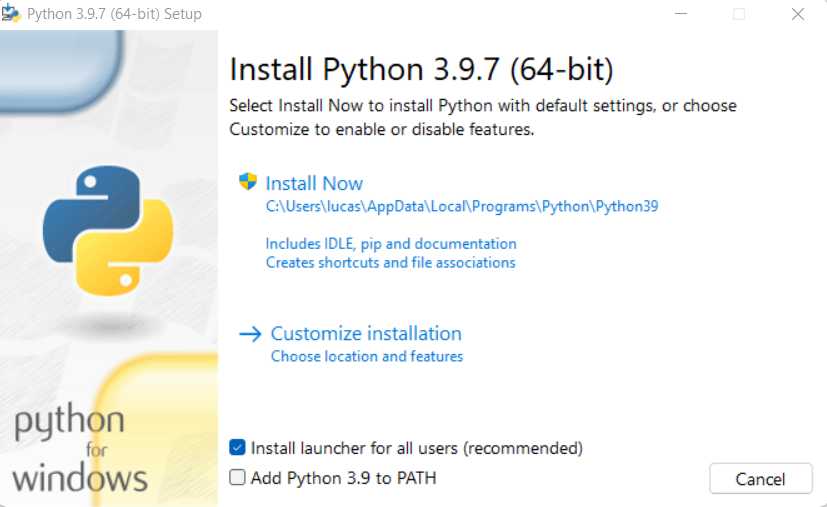
\includegraphics[scale=0.5]{instalationIDLE}
\caption{Capture d'écran lors de l'ouverture du programme d'installation}
\end{figure}

Votre premier réflexe va être de vouloir ouvrir IDLE mais plusieurs "fichier" on était installer. Vous pourriez être tenté d'ouvrir celui qui s'appelle Python 3.9 (selon la version installée). Or c'es ce qu'on appelle un terminale. Il est possible de codé dans un terminale mais ce n'est pas optimale. Nous préférerons utiliser l'éditeur IDLE en ouvrant le fichier nommée IDLE(Python 3.9.7). Pour écrire un programme, aller dans le menu "File" puis "New File".

\begin{figure}[H]

\includegraphics[scale=1]{IDLE-et-TERM}
\caption{IDLE a gauche et le Terminale Python a droite}
\end{figure}

\section*{Pycharm}
Pycharm est l'IDE de JetBrain. Personnellement je préféré Pycharm, il permets de faire de plus gros projets dans différents fichiers et de se retrouver plus facilement. En plus de cela, il nous aide a respecter la PEP8 qui est une norme visant a ce que tout les programmeur Python programmes de la même façon et puissent, par conséquent, relire le programme des autres.  \hyperref[sec:PEP8]{Nous reviendrons la dessus}.\\

\href{https://www.jetbrains.com/}{JetBrain} est un outil très utile pour les développeurs de différents langages. Il permets d'avoir des IDE pour de nombreux langages de programmations. Celui pour Python s'appelle Pycharm et est téléchargeable au lien \url{https://www.jetbrains.com/pycharm/download}. Si vous êtes étudiant, vous pouvez avoir accès au compte professionnel durant vos années d'études. Exécuter le fichier qui porte le nom pycharm-community-2021.3.2.exe (selon la version installer) et cliquer sur suivant jusqu'à l'installation. Une fois terminer, ouvrez le logiciel et accepter les conditions d'utilisation. Pour crée un programme, commencer par faire un "New Project" puis entrer le nom de votre projets. Créé un fichier en faisant un clique droit sur test en haut a gauche de la fenêtre. Sélectionner "new" puis "Python file". Nous écrirons les ici.

\begin{figure}[H]
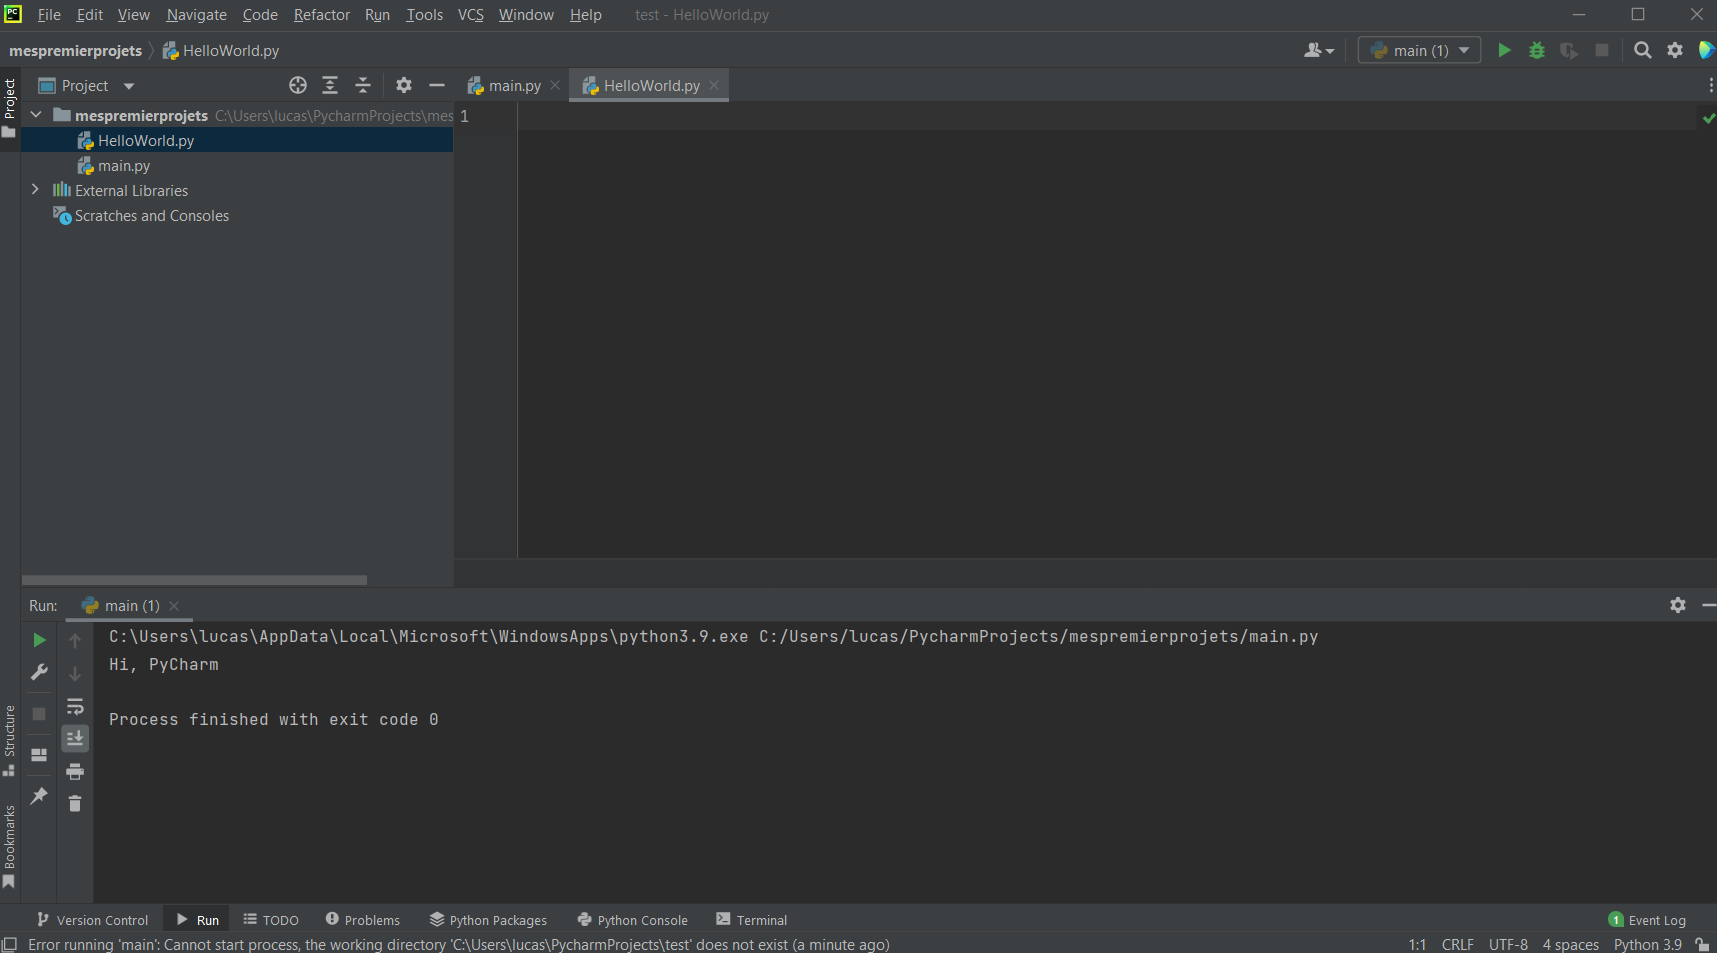
\includegraphics[scale=0.3]{Pycharm}
\caption{Capture d'écran de l'interface de Pycharm}
\end{figure}

\chapter{Quelques règle de la PEP8} \label{sec:PEP8}

Comme dit plus tôt la PEP 8 pose quelque regles qu'il est bien de suivre afin de faire un programme "propres" qui puissent etre relus par d'autres développeur facilement. Il n'est pas obligatoire de la suivre mais je vous conseille de prendre cette habitude, elle vous rendra de grands services quand vous aurez besoin d'aller sur les forums, de partager vos codes ou même lorsque vous reprendrez, après un moments, la programmation d'un projets. Vous pouvez trouver toutes les règles de la PEP 8 sur le site officiel de Python ou directement au lien \url{https://www.python.org/dev/peps/pep-0008/}. Nous allons tous de même en citer quelques unes. Vous ne les comprendrais peu être pas toutes des ce début de livres mais je vous inviterais a y revenir régulièrement.



\begin{enumerate}


	\label{PEP8:point1}\item \underline{L'indentation:} c'est la seule règle obligatoire de la PEP 8. Python n'utilise pas de commande pour la fin de ses instructions. Il est donc très important de respecter l'indentation (4 espaces) afin que le compilateur sache ce qui se trouve dans la boucle ou dans l'instruction.
	
	\label{PEP8:point2}\item \underline{Importation:} afin de savoir d'où viennent les fonctions que nous utiliserons la PEP8 conseille d'utiliser l'importation de module, de fichier et de bibliothèques avec la commande import \textit{module} plutôt que la version scolaire from \textit{module} import*. Après avoir importer les modules avec la première commande nous devrons appeler des fonction \textit{module.fonction}(), on sera donc de quelle module provient la fonction appeler. Au contraire, pour utiliser une fonction importer, avec le version scolaire, nous utiliserons la commande \textit{fonction}(), nous ne connaissons pas module ou se trouve notre fonction. Nous devrions aussi importer les modules ligne par ligne avec les modules interne a Python en premier puis les module externe et le tout trier par ordre alphabétique. Si un nom de module es trop long on peut le raccourcir en utilisant le mots clé \textit{as}
	
	\label{PEP8:point3}\item \underline{Nommage:} pour savoir ce qu'est chaque objet Python, la PEP 8 défini quelque règle:
	
	\begin{itemize}[label=\textbullet]
	
		\item Le nom des variables, module et fonction sont écrit entièrement en minuscule et les mots la contenant sont séparer par des underscore. Exemple: nom\_dune\_variable (style: snake\_case)
		
		\item Les constante doivent être écrit en majuscule séparer avec un underscore. Exemple: NOM\_DE\_LA\_CONSTANTE
		
		\item Les noms de classes et d'exceptions seront ecrits avec une lettre majuscule, seulement au debut de chaque mots. Exemple: NomDuneClasse (style: CamelCase)
		
		
	\end{itemize}
	Il faut également donner un nom qui a un sens a nos objets. On autorisera seulement les noms a 1 seules caractère pour les  compteur de boucle et compteur d'indice ou pour des coordonnée cartésienne
	
	\label{PEP8:point4} \item \underline{Les espaces:} Pour les opérateur (+, -, /, *, ==, !=, <=, not, in, and, or, \dots) on mets un espace avant est après. On ne mets pas d'espace juste après une parenthèse ouvrante ou juste avant une parenthèse fermante. Pareil pour les accolades et les. Les caractère , et : n'ont pas d'espace avant mais 1 après, sauf a l'intérieur des crochets ou on ne mettra aucun espace. On ne rajoute pas d'espace non plus pour faire jolis.
	
	\label{PEP8:point5} \item \underline{retour a la ligne:} Il arrivera parfois d'avoir a écrire une ligne de code très longues. Or la PEP 8 demande a ne pas avoir de ligne execedent la taille d'un écran, sur Pycharm cette limite est fixe a 120 caractère. Nous avons donc besoin de faire des retour a la ligne.
	
	\begin{itemize}[label=\textbullet]
	
		\item Dans une suite de commande on utilisera le antislash pour faire le retour a la ligne

		\item A l'intérieur de parenthèse, de crochet ou d'accolade nous pouvons le faire après une virgule ou un opérateur séparent 2 élément. Par exemple: fonction(element1, element2, \\ element3, element4).
		Dans lorsqu'on veux couper une chaine de caractère on ferme les guillemets on fait un retour la la ligne puis on rouvre les guillemets. Exemple: print("Je suis en train d'écrire " \\ "un très grand roman de " \\  "plusieurs milliard de page")
		
		\item A l'intérieur des triples guillemets (utiliser pour les docstring) on peu faire des retour a la ligne directement.	
		
	\end{itemize}
		
	\label{PEP8:point6} \item \underline{Ligne vide:}	 Afin de rendre le programme plus lisible, Nick Coghlan, Barry Warsaw et Guido van Rossum nous recommande de laisser des lignes vides entre chaque partie de programme. De plus, il est recommander de laisser 2 lignes vides avant les définitions de classes et de fonctions.
	
	\label{PEP8:point7} \item \underline{Commentaire:} Ils nous conseille également de mettre des commentaire afin de détailler des ligne de notre programmes. Pour crée un commentaire, nous commençons par mettre un \# puis nous insérons notre commentaire. Il est également déconseiller de mettre un commentaire en fin de ligne de commande, mais en début de ligne.
	
	\label{PEP8:point8} \item \underline{Docstring:} Les docstrings sont la pour l'utilisateur du programmes, lorsqu'il appellera la commande help(\textit{fonction}) il obtiendra l'aide (la docstring) que vous aurai écrite. Elle doivent commencer et terminer par des triple guillemets et doivent comprendre une explication de votre fonction aussi que le nom des paramètre avec leur type est leur rôle dans la fonction. Elle doit également contenir les effet de bort et les retours.
	
	\label{PEP8:point9} \item \underline{Organisation du code:} Pour faire le meilleur programmes, voici les différent éléments d'un programme dans l'ordre:
	\begin{itemize}
	[label=\textbullet]
		\item On commence avec un Docstring décrivant le programme
		\item Les credits sous cette forme\\
			\_ \_ authors \_ \_ = ("Lucas Battaglia", "Deuxieme Auteur")\\
			\_ \_ contact \_ \_ = ("developement.python@gmail.com")\\
			\_ \_ version \_ \_ = '1.0.0'\\
			\_ \_ copyright \_ \_ = "copyright"\\
			\_ \_ date \_ \_ = "2022/03"\\
		\item Les importation
		\item Les constante
		\item Les définition de classe
		\item Les définition de fonction
		\item La ligne: \textit{if \_ \_ name \_ \_ == "\_ \_ main \_ \_":} Elle correspond au début du programme principale, c'est le point d'entrée
		\item Les instruction, appel de fonction, de classe, etc.
	\end{itemize}
\end{enumerate}

Il faut savoir qu'il existe de nombreuse PEP d'on on s'est également inspirer pour écrire cette partie, notamment la PEP 257.
\part{Nos début en Python}

\chapter{Les Types de données}

\section*{Les chaines de caractères} \label{sec:Chaine}
\addcontentsline{toc}{section}{Les chaines de caractères}

\section*{Les nombre entier et flottant} \label{sec:nombre}
\addcontentsline{toc}{section}{Les nombre entier et flottant}

\section*{Les Expressions booléens} \label{sec:booleens}
\addcontentsline{toc}{section}{Les Expressions booléens}

\section*{Variables, Expressions, Instructions} \label{sec:VEX}
\addcontentsline{toc}{section}{Variables, Expressions, Instructions}

\chapter{Les boucles et instructions}

\section*{Instruction conditionnelle "If"} \label{sec:If}
\addcontentsline{toc}{section}{Instruction conditionnelle "If"}

\section*{La boucle conditionnelle "While"} \label{sec:While}
\addcontentsline{toc}{section}{La boucle conditionnelle "While"}

\section*{La boucle inconditionnelle "For"} \label{sec:for}
\addcontentsline{toc}{section}{La boucle inconditionnelle "For"}




\chapter{NOM A TROUVER}

\section*{Entrées / Sorties} \label{sec:En/sor}
\addcontentsline{toc}{section}{Entrées / Sorties}

\section*{Les fonctions} \label{sec:fonction}
\addcontentsline{toc}{section}{Les fonctions}




\chapter{Le stockage de donnée simple}

\section*{Stockage a courts termes} \label{sec:VEX}
\addcontentsline{toc}{section}{Stockage a courts termes}

\subsection*{Les Listes} \label{sec:liste}
\addcontentsline{toc}{subsection}{Les liste}

\subsection*{Les dictionnaires} \label{sec:dictionnaire}
\addcontentsline{toc}{subsection}{Les dictionnaires}

\section*{Stockage a longs termes} \label{sec:VEX}
\addcontentsline{toc}{section}{Stockage a longs termes}

\subsection*{Les fichiers} \label{sec:fichier}
\addcontentsline{toc}{subsection}{Les Fichier}










\part{Les bibliothèques}

\chapter{Nos premières bibliothèques}

\section*{La bibliothèque math}
\addcontentsline{toc}{section}{La bibliothèque math}

\section*{La bibliothèque random}
\addcontentsline{toc}{section}{La bibliothèque random}

\chapter{Les bibliothèques graphiques}

\section*{La bibliothèque Turtle}
\addcontentsline{toc}{section}{La bibliothèque Turtle}

\section*{La bibliothèque Tkinter}
\addcontentsline{toc}{section}{La bibliothèque Tkinter}

\section*{La bibliothèque Pygame}
\addcontentsline{toc}{section}{La bibliothèque Pygame}

\chapter{Les bibliothèques sonore}

\backmatter

\end{document}